\newpage

\section{Introdução}
A Maratona de Programação é um evento da Sociedade Brasileira de Computação que existe desde o ano de 1996. A Maratona nasceu das competições regionais classificatórias para as finais mundiais do concurso de programação, o International Collegiate Programming Contest, e é parte da regional sulamericana do concurso.

Ela se destina a alunos e alunas de cursos de graduação e início de pós-graduação na área de Computação e afins (Ciência da Computação, Engenharia de Computação, Sistemas de Informação, Matemática, etc). A competição promove nos estudantes a criatividade, a capacidade de trabalho em equipe, a busca de novas soluções de software e a habilidade de resolver problemas sob pressão. De ano em ano temos observado que as instituições e principalmente as grandes empresas da área têm valorizado os alunos que participam da Maratona.

Várias universidades do Brasil desenvolvem concursos locais para escolher os melhores times para participar da Maratona de Programação. Estes times competem na Maratona (e portanto na regional sulamericana) de onde os melhores serão selecionados para participar das Finais Mundiais do evento. No ano de 2018, mais de 50 mil estudantes de mais de 3000 escolas de mais de 100 países competiram em regionais em todo o planeta, e apenas 135 (cerca de 1\%) participam das Finais Mundiais do evento, no Porto, Portugal. Seis times brasileiros, dos quase de 800 participantes, estarão presentes nas finais mundiais.

Os times são compostos por três estudantes, que tentarão resolver durante 5 horas o maior número possível dos 10 ou mais problemas que são entregues no início da competição. Estes estudantes têm à sua disposição apenas um computador e material impresso (livros, listagens, manuais) para vencer a batalha contra o relógio e os problemas propostos.

Os competidores do time devem colaborar para descobrir os problemas mais fáceis, projetar os testes, e construir as soluções que sejam aprovadas pelos juízes da competição. Alguns problemas requerem apenas compreensão, outros conhecimento de técnicas mais sofisticadas, e alguns podem ser realmente muito difíceis de serem resolvidos.

O julgamento é estrito. No início da competição os competidores recebem os problemas que devem ser resolvidos. Nos enunciados dos problemas constam exemplos dos dados dos problemas, mas eles não têm acesso às instâncias testadas pelos juízes. A cada submissão incorreta de um problema (ou seja, que deu resposta incorreta a uma das instâncias dos juízes) é atribuída uma penalidade de tempo. O time que conseguir resolver o maior número de problemas (no menor tempo acumulado com as penalidades, caso haja empate) é declarado o vencedor\footnote{Está introdução foi retirada do site oficial da Maratona de Programação. \url{http://maratona.ime.usp.br/}}. 

\subsection{Dicas para a competição}
Conforme você leu, a maratona de programação geralmente ocorre no período de 5 horas ininterruptas e seu objetivo é a resolução do maior número de problemas. Como a competição ocorre em um longo tempo lhe é aconselhável um preparo físico e mental para que você suporte o estresse da competição. Crie uma rotina de programação. Inicie com alguns minutos, passe para horas e logo você estará programando por horas a fio. Reuniões antes da competição com os integrantes do time auxiliam no entrosamento da equipe. Lembre-se sempre, está é uma competição em equipe. Não tente resolver tudo sozinho pois você irá perder tempo. Existem plataformas online que simulam a competição (também chamada de Contest) ou possuem um grande acervo de problemas relacionados a ela. Podemos mencionar algumas plataformas, tais como:
\begin{itemize}
    \item Codeforces
    \item URI Online Judge
    \item UVA Online Judge
\end{itemize}

Na maratona de programação cada problema tem uma cor relacionado a ele. Quando você consegue solucionar um problema lhe é dado o balão com a cor do problema. Utilize isso a seu favor. Quando a competição é iniciada procure olhar os `Standings' gerais. Busque resolver os problemas mais fáceis. Olhe ao redor e observe a frequência de aparição das cores, observe a figura \ref{fig:balao}. Este é o método mais fácil para descobrir se um problema é fácil ou não. Se nenhuma equipe conter a cor do balão associado ao exercício o qual você julga ser fácil, revise o problema pois ele pode não ser tão simples assim.

\begin{figure}[H]
    \caption{Balões Maratona de Programação}    
    \centering
    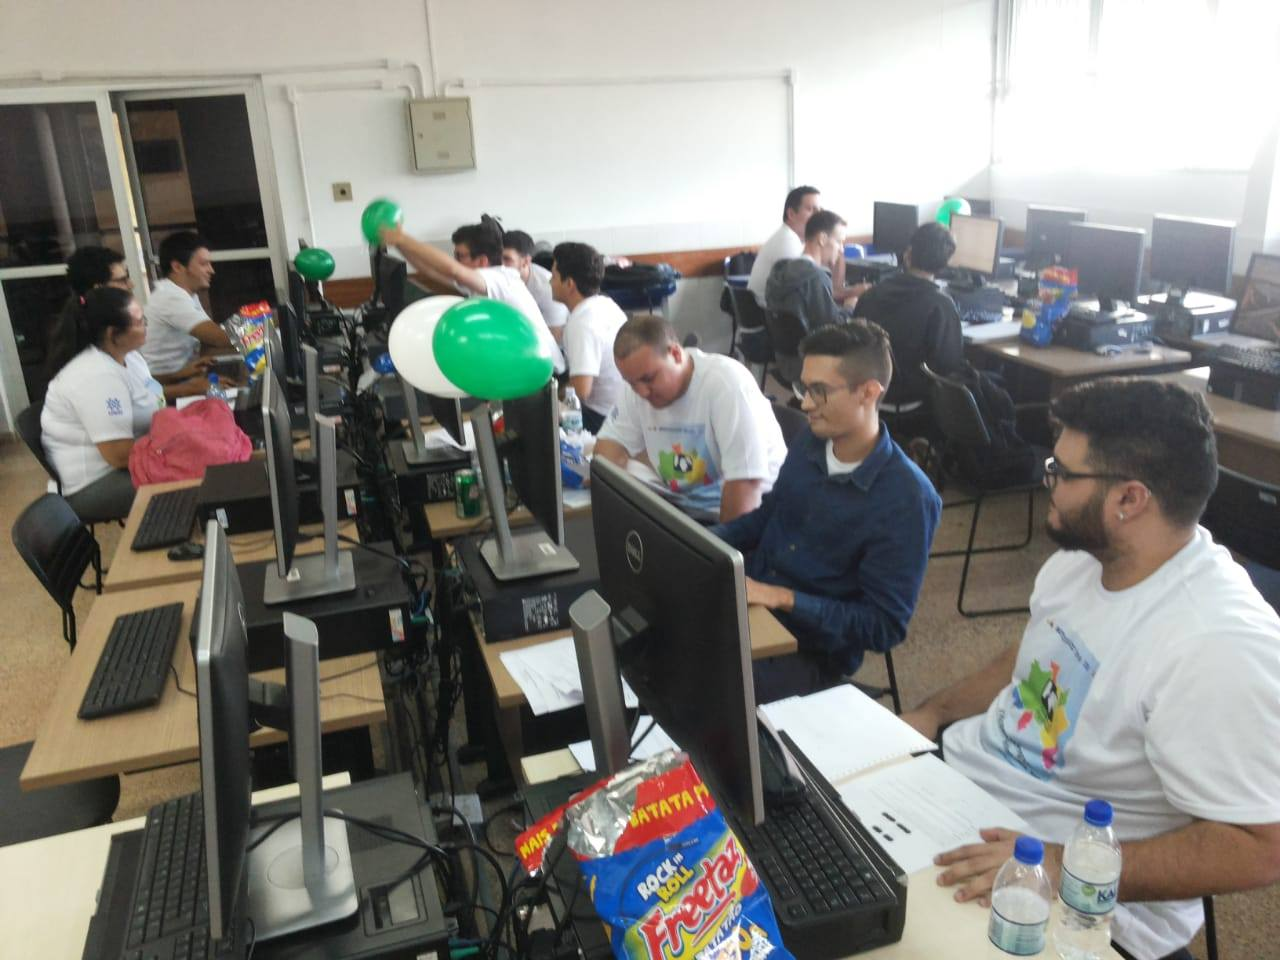
\includegraphics[scale = 0.2]{image/balao.jpg}
    \label{fig:balao}
\end{figure}
\begin{center}
    Fonte: Maratona de Programação do Norte, 2019.
\end{center}

Nas próximas seções serão abordados técnicas e problemas que comumente aparecem na competição e algumas das várias maneiras para aborda-los.



\subsection{Análise de Algoritmos} % -----------------

A eficiência dos algoritmos é importante na programação competitiva. Existem diversos problemas em que podemos facilmente supor que ele é um problema fácil. Mas usualmente, é fácil codar\footnote{Significado de codar: O ato criar códigos; programar.} um algoritmo com técnicas que resolvam o problema lentamente, mas o real desafio é inventar um algoritmo rápido. Se o algoritmo é muito lento, ele só terá pontos parciais ou nenhum ponto. Porém, ao pensarmos que é um problema fácil acabamos por aborda-lo com uma solução \textit{naive} (ingênua) por não termos o conhecimento suficiente de análise de algoritmos. 

A análise de algoritmos, estuda certos problemas computacionais recorrentes, ou seja, problemas que aparecem, sob diversos disfarces, em uma grande variedade de aplicações e de contextos. A análise de um algoritmo para um dado problema trata de:

    \begin{enumerate}
        \item Provar que o algoritmo e a técnica utilizada está correta\footnote{Utilizam-se vários métodos matemáticos, como: Indução; recorrência, etc. };
        \item Estimar o tempo que a execução do algoritmo consome;
        \item A estimativa do espaço de memória usado pelo algoritmo também é importante em muitos casos.
    \end{enumerate}
    
Conforme a literatura explana, existem três tipos de notações assintóticas estudadas na computação. Sendo elas:

    \begin{itemize}
        \item $\Omega$ - Omega
        \item $\Theta$ - Theta
        \item O - Big O
    \end{itemize}
    
Onde $\Omega$ é conhecido como o melhor caso possível, $\Theta$ caso médio, e O como pior caso. Abordaremos somente a notação Big O. Pois a análise via Big O nos permite encontrar o melhor algoritmo possível para o pior caso.
    
\subsubsection{Regras básicas para a perspectiva de cálculo de complexidade}

A complexidade de tempo de um algoritmo é denotada como O (...), onde os três pontos representam alguma função. Normalmente, a variável \textit{n} indica o tamanho da entrada. Por exemplo, se a entrada for uma matriz de números, \textit{n} será o tamanho da matriz e, se a entrada é uma string, \textit{n} será o tamanho da string.


\subsubsection*{Loops}

Por exemplo, o tempo de complexidade do código abaixo é O(\textit{n}):

\lstinputlisting[style=CPP,label={loop0},caption = {Loop em O(\textit{n})}]{algoritmos/loop_0.cpp}

E o tempo de complexidade do código abaixo é O($n^2$):

\lstinputlisting[style=CPP,label={loop1},caption = {Loop em O(\textit{n$^2$})}]{algoritmos/loop_1.cpp}

\subsubsection*{Recursão}

A complexidade de tempo de uma função recursiva depende do número de vezes a função é chamada e a complexidade de tempo de uma única chamada. O tempo total complexidade é o produto desses valores.

Por exemplo, considere a seguinte função:

\lstinputlisting[style=CPP,label={f},caption = {Função \textit{f}}]{algoritmos/f.cpp}

A chamada f(\textit{n}) causa \textit{n} chamadas de função e a complexidade de tempo de cada chamada é O(1). Assim, a complexidade total do tempo é O(\textit{n}).

Como outro exemplo, considere a seguinte função:

\lstinputlisting[style=CPP,label={g},caption = {Função \textit{g}}]{algoritmos/g.cpp}

Neste caso, cada chamada de função gera duas outras chamadas, exceto \textit{n} = 1. Veja o que acontece quando \textit{g} é chamado com o parâmetro \textit{n}. A tabela a seguir mostra as chamadas de função produzidas por esta única chamada:


\begin{table}[h!]
   \begin{center}
        \begin{tabular}{rc}
            \textbf{Função de chamada} & \textbf{Número de chamadas}\\ 
            \hline
            g(\textit{n})                       & 1                          \\
            g(\textit{n} - 1)                   & 2                          \\
            g(\textit{n} - 2)                   & 3                            \\
            ...                        & ...                           \\
            g(1)                       &2$n-1$              \\
            \hline
        \end{tabular}
         \caption{Chamadas da função \textit{g}}
         \label{tab:g}
    \end{center}
\end{table}

Com base nisso, a complexidade do tempo é:
1 + 2 + 4 + ... + 2$n-1$ = 2$^n$ - 1 = O(2$^n$).

\subsubsection{Classes de complexidade}

A lista a seguir contém complexidades de tempo comuns de algoritmos:

\begin{itemize}

    \item O(1): O tempo de execução de um algoritmo de \textbf{tempo constante} não depende do tamanho de entrada. Um algoritmo típico de tempo constante é uma fórmula direta que calcula a resposta.

    \item O(log \textit{n}): Um algoritmo \textbf{logarítmico} geralmente divide o tamanho da entrada em cada etapa. O tempo de execução de tal algoritmo é logarítmico, porque log$_2$\textit{n} é igual ao número de vezes \textit{n} deve ser dividido por 2 para obter 1.

    \item O($\sqrt{\textit{n}}$): Um algoritmo de \textbf{raiz quadrada} é mais lento que O(log \textit{n}), mas é mais rápido que O(\textit{n}). Uma propriedade especial de raízes quadradas é que $\sqrt{\textit{n}}$ = n / $\sqrt{\textit{n}}$ , então a raiz quadrada $\sqrt{\textit{n}}$ mentiras, em certo sentido, no meio da entrada.

    \item O(\textit{n}): Um algoritmo \textbf{linear} passa pela entrada um número constante de vezes. Este é geralmente a melhor complexidade de tempo possível, porque geralmente é necessário acesse cada elemento de entrada pelo menos uma vez antes de relatar a resposta.

    \item O(\textit{n} log \textit{n}): Essa complexidade de tempo geralmente indica que o algoritmo classifica a entrada, porque a complexidade de tempo dos algoritmos de ordenação eficientes é O(\textit{n} log \textit{n}). Outra possibilidade é que o algoritmo use uma estrutura de dados onde cada a operação leva tempo O(log \textit{n}).

    \item O($n^2$): Um algoritmo \textbf{quadrático} geralmente contém dois loops aninhados. É possível percorrer todos os pares dos elementos de entrada no tempo O($n^2$).

    \item O($n^3$): Um algoritmo \textbf{cúbico} geralmente contém três loops aninhados. É possível ir através de todas as trincas dos elementos de entrada no tempo O($n^3$).

    \item O(2$^n$): Essa complexidade de tempo geralmente indica que o algoritmo itera todos os subconjuntos dos elementos de entrada. Por exemplo, os subconjuntos de {1, 2, 3} são , {1}, {2}, {3}, {1, 2}, {1, 3}, {2, 3} e {1, 2, 3}.

    \item O(\textit{n}!): Essa complexidade de tempo geralmente indica que o algoritmo itera todas as permutações dos elementos de entrada. Por exemplo, as permutações de {1, 2, 3} são (1, 2, 3), (1, 3, 2), (2, 1, 3), (2, 3, 1), (3, 1, 2) e (3 2, 1).

\end{itemize}

Um algoritmo é polinomial se sua complexidade de tempo for no máximo O(n $^k$) onde \textit{k} é uma constante. Todas as complexidades de tempo acima, exceto O(2$^n$) e O(\textit{n}!), são polinomiais. Na prática, a constante \textit{k} é geralmente pequena e, portanto, um tempo polinomial complexidade significa que o algoritmo é eficiente. 

A maioria dos algoritmos nesta apostila é polinomial. Ainda assim, existem muitos problemas para os quais nenhum algoritmo polinomial é conhecido, ou seja, ninguém sabe como resolvê-los eficientemente. Os problemas NP-difíceis são um conjunto importante de problemas, qual nenhum algoritmo polinomial é conhecido\footnote{Um livro clássico sobre o tema : M. R. Garey’s and D. S. Johnson’s Computers and Intractability:
A Guide to the Theory of NP-Completeness}

%----------------

\subsubsection{Soma máxima de um subvetor}
    
Muitas vezes há vários algoritmos possíveis para resolver um problema de modo que as complexidades do tempo são diferentes. Esta seção discute um problema clássico que tem uma solução direta O(n$^3$). No entanto, projetando um algoritmo melhor, é possível resolver o problema no tempo O(\textit{n}$^2$) e até no tempo O(\textit{n}).    

Dado um vetor de \textit{n} números, nossa tarefa é calcular o máximo de soma dos raios, isto é, a maior soma possível de uma sequência de valores consecutivos no vetor 2. O problema é interessante quando pode haver valores negativos no
vetor. Por exemplo, no vetor: $ [-1, 2, 4, -3, 5, 2, -5, 2]$,

A soma máxima desse vetor é 10.

\subsubsection{Algoritmo 1}

Uma maneira simples de resolver o problema é percorrer todos os sub-argumentos possíveis, calcule a soma dos valores em cada subvetor e mantenha a soma máxima. O código a seguir implementa esse algoritmo:

\lstinputlisting[style=CPP,label={algoritmo1},caption = {Algoritmo 1 em O(\textit{n}$^3$)}]{algoritmos/algoritmo_1.cpp}

As variáveis \textit{a} e \textit{b} fixam o primeiro e último índice do subvetor, e o soma dos valores é calculada para a soma variável. A variável melhor contém o soma máxima encontrada durante a pesquisa. A complexidade temporal do algoritmo é O(\textit{n}$^3$), porque consiste em três loops aninhados que passam pela entrada.

\subsubsection{Algoritmo 2}

É fácil tornar o Algoritmo 1 mais eficiente removendo um loop dele. Isto é possível calculando a soma ao mesmo tempo quando a extremidade direita do movimentos subvetor. O resultado é o seguinte código:

\lstinputlisting[style=CPP,label={algoritmo2},caption = {Algoritmo 2 em O(\textit{n}$^2$)}]{algoritmos/algoritmo_2.cpp}


Após essa alteração, a complexidade do tempo é O(\textit{n}$^2$).

\subsubsection{Algoritmo 3}

Surpreendentemente, é possível resolver o problema em tempo O(\textit{n}), o que significa que apenas um loop é suficiente. A ideia é calcular, para cada posição do vetor, soma máxima de um subvetor que termina nessa posição. Depois disso, a resposta para o problema é o máximo dessas somas. Considere o subproblema de encontrar o subvetor de soma máxima que termina em posição \textit{k}. Existem duas possibilidades:

    \begin{enumerate}
        \item O subvetor contém apenas o elemento na posição \textit{k}.
        \item O subvetor consiste em um subvetor que termina na posição \textit{k} - 1, seguido por o elemento na posição \textit{k}.
    \end{enumerate}

Neste último caso, uma vez que queremos encontrar um subvetor com soma máxima, o subvetor que termina na posição \textit{k} - 1 também deve ter a soma máxima. Portanto, podemos resolver o problema de forma eficiente, calculando a soma máxima de subvetor para cada posição final da esquerda para a direita. O código a seguir implementa o algoritmo:

\lstinputlisting[style=CPP,label={algoritmo3},caption = {Algoritmo 3 em O(\textit{n})}]{algoritmos/algoritmo_3.cpp}
      

O algoritmo contém apenas um loop que passa pela entrada, então o tempo complexidade é O(\textit{n}). Esta é também a melhor complexidade de tempo possível, porque qualquer algoritmo para o problema tem que examinar todos os elementos da matriz pelo menos uma vez.

\subsubsection{Comparação de eficiência}

É interessante estudar como os algoritmos eficientes são na prática. Os seguintes tabela mostra os tempos de execução dos algoritmos acima para diferentes valores de \textit{n} em um computador moderno. Em cada teste, a entrada foi gerada aleatoriamente. O tempo necessário para a leitura a entrada não foi medida.

\begin{table}[H]
   \begin{center}
        \begin{tabular}{csrrr}
            \textbf{Tamanho de \textit{n}} & \textbf{Algoritmo 1} & \textbf{Algoritmo 2} & \textbf{Algoritmo 3}\\ 
            \hline
            10$^2$ &   0.0 s & 0.0 s & 0.0 s \\
            10$^3$ &   0.1 s & 0.0 s & 0.0 s \\
            10$^4$ & > 10.0 s & 0.1 s & 0.0 s \\
            10$^5$ & > 10.0 s & 5.3 s & 0.0 s \\
            10$^6$ & > 10.0 s & > 10.0 s & 0.0 s \\
            10$^7$ & > 10.0 s & > 10.0 s & 0.0 s \\
            \hline
        \end{tabular}
         \caption{Aoooooooooooooooooo 35}
         \label{tab:complexidade}
    \end{center}
\end{table}

A comparação mostra que todos os algoritmos são eficientes quando o tamanho da entrada é insumos pequenos, mas maiores, trazem diferenças notáveis nos tempos de execução dos algoritmos. Algoritmo 1 torna-se lento quando \textit{n} = 10 $^4$ e Algoritmo 2 torna-se lento quando \textit{n} = 10$^5$. Apenas o Algoritmo 3 é capaz de processar até mesmo os maiores entradas instantaneamente.


\begin{comment}
Para que possa entender melhor o que é o Big O imagine o seguinte caso: 
\lstinputlisting[style=CPP,label={O(n)},caption = {Algoritmo O(n)}]{algoritmos/primeiro.cpp}
\end{comment}


\rule{\textwidth}{0.4pt}
\large{\textbf{Exercícios\footnote{Os exercícios encontram-se disponíveis na plataforma URI Online Judge. \url{htps://www.urionlinejudge.com.br}}}}\\

\begin{itemize}
    \item \textbf{1221} - Primo Rápido
    \item \textbf{1424} - Problema Fácil de Rujia Liu?
    \item \textbf{1805} - Soma Natural
\end{itemize}

\newpage